%-------------------------------------------------------------------------------
\section{Methodology}
%-------------------------------------------------------------------------------
In order to confirm the findings presented in Fu et.al.\cite{Fu}, we deployed our 
own instance of their autofz environment. We replicated their testing environment 
by deploying their docker image on our own hardware. Moreover, we tested our 
recreation of Fu et al.'s autofz against the targets: exiv2, mp3gain, mojs, and 
tcpdump. Our initial findings validate the results presented in Fu et al.; autofz 
is consistently a top performing  against the tested targets.

We have also been able to produce a working tool chain on ARM64, with some significant 
variations from Fu et al. \cite{Fu}. Our ARM64 environment implements 7 fuzzing 
algorithms in Ubuntu 22.04 LTS, running in a virtual machine with the UTM app on 
host laptops running macOS 14.3.1 on Apple Silicon (ARM64) architecture 
\textbf{(RQ1)}. Key differences are described in Table \ref{arm64-characteristics}.

\begin{table}[ht]
    \begin{tabular}{|l|l|l|l|}
        \hline
                        & Original\cite{Fu} & ARM64 & Reason \\
        \hline
        Ubuntu Version  & 16.04             & 22.04 & 1 \\
        \hline
        aflforkserver.so    & x86\_64           & aarch64 & 2 \\
        \hline
        AFL (original)  & Yes               & Yes & \\
        \hline
        AFLFast         & Yes               & Yes & \\
        \hline
        Angora          & Yes               & No & 4 \\
        \hline
        Fairfuzz        & Yes               & Yes & \\
        \hline
        LAF-Intel       & Yes               & Yes & \\
        \hline
        LearnAFL        & Yes               & No & 3 \\
        \hline
        LibFuzzer       & Yes               & Yes & \\
        \hline
        QSYM            & Yes               & No & 4 \\
        \hline
        Radamsa         & Yes               & Yes & \\
        \hline
        RedQueen        & Yes               & Yes & \\
        \hline
    \end{tabular}
    \caption{Key differences between Original AMD64 and ARM64 Environments}
    \label{arm64-characteristics}
\end{table}

There are a number of reasons for the differences between Fu et al.,
and our ARM64 environment. They correspond to the reason numbers in Table 
\ref{arm64-characteristics} and are:

\begin{enumerate}
    \item Ubuntu 16.04 LTS does not support the ARM64 architecture (also called 
    aarch64).
    \item Aflforkserver.so comes from the quickcov package, developed to support 
    the Cupid research project\cite{guler2020cupid}. We had to recompile it for aarch64.
    \item Learn AFL does not properly compile instrumented binaries for aarch64.
    \item Angora and QSYM are written such that they are dependent upon the x86\_64 ISA.
    They do not support other architectures.
\end{enumerate}

To compare the  modified autofz with the proposed autofz, we tested it against the 
targets: exiv2, nm, mojs, and tcpdump. Initial test indicate that the ARM64 compatible 
autofz performs similarly to the unmodified autofz. Figure \ref{fig:exiv2_compare_orig_arm64} 
displays bitmap density covered of the individual algorithms in our ARM64 implementation, 
as compared to a similar plot from Fu et. al\cite{Fu}.

\begin{figure}
    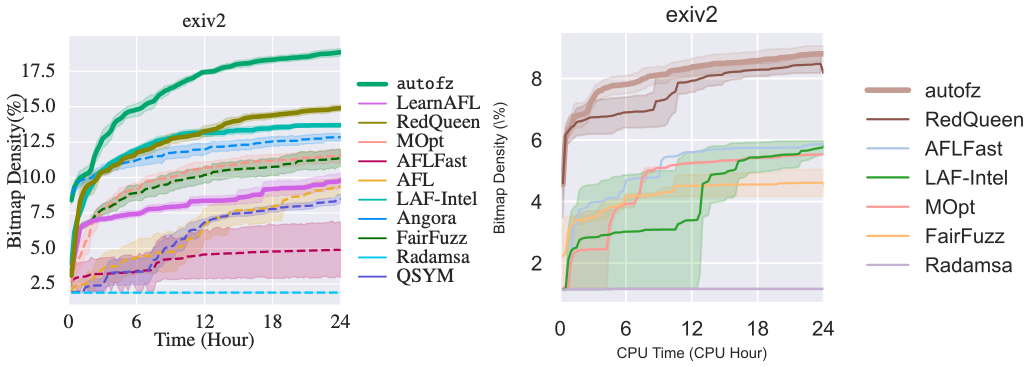
\includegraphics[width=0.52\textwidth]{figs/exiv2_compare_orig_arm64.png}
    \centering
    \caption{A comparison of bitmap density covered in the original\cite{Fu} and our 
    coverage during initial fuzzing of exiv2}
    \label{fig:exiv2_compare_orig_arm64}
\end{figure}

Bitmap density coverage of our initial fuzzing campaign against tcpdump is plotted 
in figure \ref{fig:tcpdump_bmdensity_8Mar2024}, shown as a comparison with results 
from Fu et al.\cite{Fu}.

In addition to producing an ARM64 compatible autofz, we identified a potential improvement for autofz.
Existing versions of autofz use bitmap coverage to rank fuzzers during the preparation, but bitmap
coverage may not be the best metric for identifying the most effective fuzzers for a target. While
bitmap coverage indicates the portion of a target that was fuzzed, it does not guarantee bug discovery.
To resolve these problems, we plan to modify autofz, so fuzzers that discover more bugs during the
preparation phase are rewarded with more resources during the focus phase because discovering more bugs
across a smaller area of code decreases the attack surface by more entry points than discovering fewer
bugs over a greater area of the code.